% !TEX encoding = UTF-8 Unicode
\documentclass[a4paper]{article}

\usepackage{color}
\usepackage{url}
\usepackage[T2A]{fontenc} % enable Cyrillic fonts
\usepackage[utf8]{inputenc} % make weird characters work
\usepackage{graphicx}
\graphicspath{ {images/} }

\usepackage[english,serbian]{babel}
%\usepackage[english,serbianc]{babel} %ukljuciti babel sa ovim opcijama, umesto gornjim, ukoliko se koristi cirilica

\usepackage[unicode]{hyperref}
\hypersetup{colorlinks,citecolor=green,filecolor=green,linkcolor=blue,urlcolor=blue}

\usepackage{listings}

\usepackage{amsmath}
\usepackage{amsfonts}

% https://tex.stackexchange.com/questions/5223/command-for-argmin-or-argmax
\DeclareMathOperator*{\argmax}{argmax}

%\newtheorem{primer}{Пример}[section] %ćirilični primer
\newtheorem{primer}{Primer}[section]

\definecolor{mygreen}{rgb}{0,0.6,0}
\definecolor{mygray}{rgb}{0.5,0.5,0.5}
\definecolor{mymauve}{rgb}{0.58,0,0.82}

\lstset{ 
  backgroundcolor=\color{white},   % choose the background color; you must add \usepackage{color} or \usepackage{xcolor}; should come as last argument
  basicstyle=\scriptsize\ttfamily,        % the size of the fonts that are used for the code
  breakatwhitespace=false,         % sets if automatic breaks should only happen at whitespace
  breaklines=true,                 % sets automatic line breaking
  captionpos=b,                    % sets the caption-position to bottom
  commentstyle=\color{mygreen},    % comment style
  deletekeywords={...},            % if you want to delete keywords from the given language
  escapeinside={\%*}{*)},          % if you want to add LaTeX within your code
  extendedchars=true,              % lets you use non-ASCII characters; for 8-bits encodings only, does not work with UTF-8
  firstnumber=1000,                % start line enumeration with line 1000
  frame=single,	                   % adds a frame around the code
  keepspaces=true,                 % keeps spaces in text, useful for keeping indentation of code (possibly needs columns=flexible)
  keywordstyle=\color{blue},       % keyword style
  language=Python,                 % the language of the code
  morekeywords={*,...},            % if you want to add more keywords to the set
  numbers=left,                    % where to put the line-numbers; possible values are (none, left, right)
  numbersep=5pt,                   % how far the line-numbers are from the code
  numberstyle=\tiny\color{mygray}, % the style that is used for the line-numbers
  rulecolor=\color{black},         % if not set, the frame-color may be changed on line-breaks within not-black text (e.g. comments (green here))
  showspaces=false,                % show spaces everywhere adding particular underscores; it overrides 'showstringspaces'
  showstringspaces=false,          % underline spaces within strings only
  showtabs=false,                  % show tabs within strings adding particular underscores
  stepnumber=2,                    % the step between two line-numbers. If it's 1, each line will be numbered
  stringstyle=\color{mymauve},     % string literal style
  tabsize=2,	                   % sets default tabsize to 2 spaces
  title=\lstname                   % show the filename of files included with \lstinputlisting; also try caption instead of title
}

\begin{document}

\title{Automatsko prepoznavanje govora\\ \small{Seminarski rad u okviru kursa\\Metodologija stručnog i naučnog rada\\Matematički fakultet}}

\author{Vladimir Vuksanović, Aleksa Kojadinović, Lazar Čeliković\\kontakt email prvog, drugog, trećeg autora}

%\date{9.~april 2015.}

\maketitle

\abstract{
U ovom tekstu je ukratko prikazana osnovna forma seminarskog rada. Obratite pažnju da je pored ove .pdf datoteke, u prilogu i odgovarajuća .tex datoteka, kao i .bib datoteka korišćena za generisanje literature. Na prvoj strani seminarskog rada su naslov, apstrakt i sadržaj, i to sve mora da stane na prvu stranu! Kako bi Vaš seminarski zadovoljio standarde i očekivanja, koristite uputstva i materijale sa predavanja na temu pisanja seminarskih radova. Ovo je samo šablon koji se odnosi na fizički izgled seminarskog rada (šablon koji \emph{morate} da koristite!) kao i par tehničkih pomoćnih uputstava. Pročitajte tekst pažljivo jer on sadrži i važne informacije vezane za zahteve obima i karakteristika seminarskog rada.}
% Tema ovog rada je da priblizi citaoca zadatku automatskog prepoznavanja govora, problemima koji se javljaju i najznacajnijim arhitekturama ovih sistema.

\bigskip
\textbf{Ključne reči:} prepoznavanje govora

\tableofcontents

\newpage

\section{Uvod}
\label{sec:uvod}

Govor je za ljude najintuitivniji i prirodniji nacin komunikacije. Zbog toga je od samog nastanka kompjutera, nastala i ideja da koristimo isti nacin komunikacije da interagujemo sa njima.
To bi znatno smanjilo potrebno predznanje za koriscenje kompjutera i ucnilio ga pristupacnijim vecem broju ljudi. Najveca prepreka ovim sistemima do skoro je bio kako sa velikom tacnosti prepoznati sta je korisnik rekao.
Taj postupak se naziva automatsko prepoznavanje govora.

\textbf{Automatsko prepoznavanje govora} (eng.~{\em Automatic Speech Recognition, ASR}) je proces pretvaranja zvučnog signala govora u sekvencu reči pomoću kompjutera.
Neke od najznacajnijih primena ovih sistema su: pametni licni asistenti (Google Assistant\footnote{https://assistant.google.com/}, Apple Siri\footnote{https://www.apple.com/siri/},\dots), transkripcija snimaka, pretrazivanje audio sadrzaja i pristupacnost.
% slika waveform u recenicu (Uday 8.1) ?

Iako su istrazivanja na ovu temu pocela jos sredinom dvadesetog veka, popularnost je pocela da dobija tek u poslednjoj deceniji kada je uvodjenje dubokih neuronskih mreza drasticno povecalo performanse ovih sistema.
Ta razlika je bila dovoljna da ucini ove sisteme prakticno primenljivim umesto nezgodnim za upotrebu zbog velikog broja gresaka.
Jedan od najznacajnijih postignuca je ostvareno 2016. godine je kompanija Majkrosoft napravila sistem koji je ostvario iste rezultate kao ljudski eksperti na transkripciji Switchboard skupa podataka \cite{switchboard}.
% Human level switchboard
% https://blogs.microsoft.com/ai/historic-achievement-microsoft-researchers-reach-human-parity-conversational-speech-recognition/
% https://www.microsoft.com/en-us/research/blog/microsoft-researchers-achieve-new-conversational-speech-recognition-milestone/
Za glavne uzroke ovog naglog poboljsanja se smatraju \cite{hannun2021history}:
\begin{enumerate}
  \item Sakupljanje velike kolicine tanskribovanih skupova podataka
  \item Nagli porast u performansama grafickih procesorskih jedinica (GPU)
  \item Poboljsanje algoritama za ucenje i arhitektura modela
\end{enumerate}
% The History of Speech Recognition to the Year 2030
% 1) the curation of massive transcribed data sets,
% 2) the rapid rate of progress in graphics processing units
% 3) the improvement in the learning algorithms and model architectures.

% izlistati poglavlja
U nastavku cemo prvo navesti neke izazove koje treba da resimo da bi smo napravili dobar sistem za prepoznavanje govora, zatim cemo opisati nacin rada dva najpopularnija modela: statisticki i end-to-end i na kraju cemo predstaviti nacin za njihovu evaluaciju.

\section{Izazovi}
% https://www.youtube.com/watch?v=q67z7PTGRi8
Prepoznavanje govora je veoma tezak zadatak zato sto je potrebno da radi podjednako dobro u veoma razlicitim uslovima.
Neki od najvecih izazova su:
\begin{itemize}
  \item \textbf{Mala kolicina podataka za trening} --- 
  Za ostvarivanje dobrih rezultata potrebno je sakupiti vise stotina ili cak hiljada sati labeliranih zvucnih snimaka koji treba da sadrze vise govornika razlicitog pola i starosti, koji govore razlicitim akcentima. 
  Dok u skorije vreme jeste nastao porast u kolicini dostupnih podataka, veliki problem jos uvek predstavlja reprezentativnost razlicitih varijacija u govoru i nedostatak podataka za jezike sa manjim brojem govornika. 
  Zbog toga se istrazuju alternativni nacini za treniranje kao sto su samo-treniranje (eng.~{\em self-training}) \cite{baevski2020wav2vec}, iterativno treniranje \cite{park2020noisy} ili treniranje koristeci kompjuterski generisan glas \cite{hannun2014deep}. 
  U dodatku \ref{sec:skupovi} se moze naci tabela sa pregledom nekih od najpopularnijih trening skupova na engleskom jeziku.
  
  \item \textbf{Stil govora} --- 
  Postoje razliciti sistemi u zavisnosti od toga koji tip govora mogu da prepoznaju \cite{anusuya2010speech}. Tipovi govora poredjani po tezini propoznavanja su: 
  \begin{enumerate}
    \item Izolovane reci --- reci su razdvojene dugim periodima tisine
    \item Povezane reci --- reci su razdvojene kratkim pauzama
    \item Neprekidan govor --- uvezbani govor, citanje ili diktiranje
    \item Spontan govor --- neuvezbani, prirodni govor 
  \end{enumerate}
  Prve implementacije prepoznavanja govora su radile na nivou izolovanih reci i koristile su se za prepoznavanje odredjenih komandi ili cifara.
  Danas se najvise truda ulaze u poboljsanje neprekidnog i spontanog govora.

  \item \textbf{Karakteristike govornika} ---
  Svaki covek ima razlicitu boju glasa i govori razlicitom brzinom. Cak i starost osobe i jacina govora bitno uticu na frekvenciju glasa.
  Poseban problem pravi postojanje razlicitih dijalekata i akcenata koji mogu da imaju potpuno razlicite nacine za izgovaranje istih reci.
  Jedan nacin za resavanje ovog problema je treniranje sistema na glasu govornika koji ce ga koristiti.
  To su sistemi zavisni od korisnika (eng.~{\em speaker dependent}) i koriste se u slucajevima da samo jedno osoba treba da ih koristi.
  Sa druge strane postoje sistemi nezavisni od korisnika (eng.~{\em speaker independent}) koji treba da rade podjednako dobro za sve govornike.
  
  \item \textbf{Okruzenje govornika} --- 
  Ovi sistemi ce retko biti korisceni u potpuno tihim prostorijama sa profesionalnom opremom za snimanje, zbog toga treba da budu tolerantni na razlicite vrste pozadinske buke ili kvaliteta mikrofona (koliko je to moguce). 
  Neke vrste sumova je moguce otkloniti analizom zvuka ili naprednijim metodama \cite{xu2015enhancement}, ali jedan od najvecih problema predstavlja postojanje drugih govornika u okolini.
  Te signale je cesto tesko razlikovati od glasa primarnig govornika, i samim tim tesko ukloniti.
  
  \item \textbf{Velicina recnika} --- 
  Povecanje broja reci koje model moze da prepozna takodje povecava njegovu slozenost i otezava treniranje, ali se time dobija na tacnosti. 
  Zbog toga je potrebno naci dobar kompromis izmedju velicine recnika i slozenosti modela. 
  U slucajevima kada je potrebno pouzdano prepoznati samo neki skup komandi koriste se mali recnici i oni su cesto veoma pouzdani, ali za prepoznavanje opsteg govora danasnji sistemi su trenirani na skupu od oko 50.000-100.000 reci.
\end{itemize}

\section{Statisticki model}
% Uday knjiga chap. 8
Dugo vremena statisticki pristup je bio dominantan za sisteme za prepoznavanje govora.
Cilj ovih sistema je da pronadju najverovatniju transkripciju za zadati ulaz.
% Large Vocabulary Continuous Speech Recognition a Review
Formalno, neka je $\hat{W}$ optimalan niz reci za transkripciju nekog zvucnog signala $X$. Cilj je optimizovati formulu \cite{kamath2019nlp}:
\begin{equation*}
  \hat{W} = \argmax_{W} P(W|X)
\end{equation*}
primenom Bajesove formule to mozemo da zapisemo kao:
\begin{equation*}
  \hat{W} = \argmax_{W} \frac{P(X|W) P(W)}{P(X)}
\end{equation*}
a kako je $P(X)$ konstantno za konkretan ulaz, mozemo da ga eliminisemo:
\begin{equation}
  \label{eq:stat1}
  \hat{W} = \argmax_{W} P(X|W) P(W)
\end{equation}
Prvi deo, $P(X|W)$, racuna \textbf{akusticki model} (eng.~{\em acoustic model}), a drugi, $P(W)$, racuna \textbf{jezicki model} (eng.~{\em language model}).
Ideja je da odvojeno optimizujemo obe prethodne velicine i ocekujemo da ce se tako maksimizirati ukupna verovatnoca.

Najprirodniji nacin za racunanje $P(X|W)$ bi bio na nivou reci zato sto krajnji izlaz svakako treba da bude niz reci.
Problem sa tim je sto postoji veliki broj varijacija u izgovoru reci, a nedovoljan broj primera za svaki od njih u trening skupu.
Umesto toga, reci se dele na manje delove kao sto su foneme.
\textbf{Foneme} su najmanje jezicke jedinice cijom kombinacijom se dobijaju reci. One postoje samo kao apstraktna ideja a njihova fizicka realizacija se zove glas.

Znaci ako je $S$ niz fonema, $P(X|W)$ iz formule \ref{eq:stat1} se razlaze i dobija se:
\begin{equation*}
  \hat{W} = \argmax_{W} \sum_{S} P(X,S|W) P(W)
\end{equation*}
sto se moze aproksimirati kao:
\begin{equation}
  \label{eq:stat2}
  \hat{W} \approx \argmax_{W,S} P(X|S) P(S|W) P(W)
\end{equation}
gde se $P(S|W)$ zove \textbf{model izgovora} (eng.~{\em pronunciation model}). 

% slika modela
% https://www.idiap.ch/software/bob/docs/bob/bob.kaldi/stable/_images/ASR.png
Na slici \ref{fig:statistical_model} je prikazana cela struktura statistickog modela od zvucnog signala do transkripcije:
\begin{figure}[h!]
  \begin{center}
    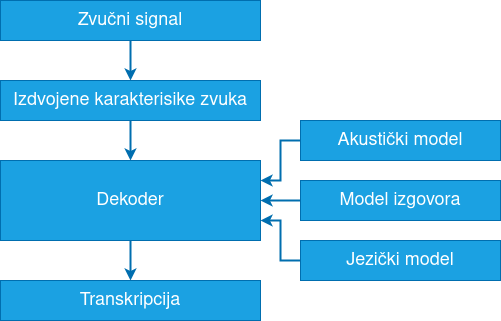
\includegraphics[scale=0.4]{statistical_model.png}
  \end{center}
  \caption{Statisticki model}
  \label{fig:statistical_model}
\end{figure}

U nastavku ce biti opisana svaka od pomenutih komponenti, njena uloga i nacin rada.

\subsection{Procesiranje zvucnog signala}
Sirovi zvucni signal je veoma nepogodan za koriscenje zato sto sadrzi veliku kolicinu nepotrebnih informacija i šuma.
Zbog toga se pre prosledjivanja akustickom modelu, signal prvo obradjuje tako da ostanu samo kljucne karakteristike i smanji sum i velicina reprezentacije.

Signal delimo na kratke segmente koje zovemo \textbf{okviri} (eng.~{\em frame}).
Svaki od njih je fiksne duzine (obicno 10-30 milisekundi) sa kratkim preklapanjem susednim okvirima radi smanjenja naglih promena prilikom prelaska iz jednog u drugi.
Pretpostavka je da je u svakom od okviru glas konstantan, to jest da se glasovi mogu menjati samo prelaskom iz jednog okvira u drugi.
Na svaki od tih novodobijenih delova se zatim primenjuje neka vrsta spektralne analize najcesce zasnovana na Furijeovoj transformaciji kojom se izdvajaju samo njegove najbitnije karakteristike.
Izdvajanje karakteristika pokusava da oponasa ljudski slusni sistem filtrirajuci odredjene frekvencije i skalirajuci ih onako kako bi ih covek cuo.
Tacna reprezentacija koja se koristi varira u zavisnosti od modela, ali jedna od najpopularnijih je MFCC [?].

\subsection{Akusticki model}
% https://www.cs.cmu.edu/~roni/10601-slides/hmm-for-asr-whw.pdf
% https://ocw.mit.edu/courses/electrical-engineering-and-computer-science/6-345-automatic-speech-recognition-spring-2003/lecture-notes/lecture15.pdf
Akusticki model je zaduzen da pretvori obradjeni zvucni signal u sekvencu fonema. 
Za resavanje ovog problema uvescemo teoriju o skrivenim Markovljevim modelima \cite{rabiner1989hmm}.

% https://cs229.stanford.edu/section/cs229-hmm.pdf
Neka je $S = \{s_1, s_2, \dots, s_n\}$ skup stanja, $A$ matrica dimenzije $n \times n$ gde $A_{ij}$ predstavlja verovatnocu prelaska iz stanja $s_i$ u $s_j$ tako da vazi $A_{ij} > 0$ i $\sum_{j=1}^{n} A_{ij} = 1$.
U diskretnim trenucima vrsi se promena trenutnog stanja na osnovu verovatnoca zadatih matricom $A$. 
Specijalno, pocetno stanje moze da se izabere nasumicno iz neke raspodele.
Za svaki trenutak $t = 1,2,\dots,T$, oznacicemo stanje u tom trenutku sa $q_t$.
Ukoliko dodatno vazi da verovatnoca prelaska u sledece stanje vazi samo od trenutnog stanja: 
$$P(q_t = S_i | q_{t-1} = S_j, q_{t-2} = S_k, \dots) = P(q_t = S_i | q_{t-1} = S_j)$$
i da se verovatnoce prelaska iz jednog stanja u drugo ne menjaju:
$$P(q_t = S_i | q_{t-1} = S_j) = P(q_2 = S_i | q_1 = S_j) \forall t=2..T$$
onda se prethodno opisan sistem naziva \textbf{Markovljev model}.

Prosirimo sada ovaj sistem dalje. Neka vaze sve prethodno uvedene oznake i dodatno neka je $V = \{v_1, v_2, \dots, v_m\}$ skup mogucih obzervacija za svako stanje i $B$ matrica dimenzije $n \times m$ gde $B_{jk}$ predstavlja verovatnocu obzervacije $v_k$ u stanju $s_j$.
Sada u svakom trenutku $t$ osim promene stanja dobijamo i novu obzervaciju $x_t$ na osnovu verovatnoca zadatih matricom $B$.
Razlika sada je sto novo stanje ostaje skriveno nego se samo vidi obzervacija u svakom trenutku.
Ako jos vazi da je svaka obzervacija zavisi samo od trenutnog stanja a ne od prethodnih obzervacija:
$$P(x_t = v_i | x_{t-1}, \dots, x_1, q_t, \dots, q_1) = P(x_t = v_i | q_t)$$
tada se ovaj sistem se naziva \textbf{skriveni Markovljev model}.

Konkretno za prepoznavanje govora koristicemo ove modele da opisemo svaku fonemu.
Svaki od njih ce se sastojati od nekog zadatog broja stanja pri cemu ce obzervacije govoriti da li je ta fonema trenutno primecena.
Kada imamo model za svaku fonemu, njih je moguce kombinovati da se dobije model za rec, koji se dalje kombinuju u model za recenicu.
Sada jos samo treba odrediti raspodele verovatnoca za obzervacije fonema. 
To se radi treniranjem modela nad skupom podataka uz pomoc Baum-Welch algoritma zasnovanog na dinamickom programiranju.

Istrenirani model posle moze da predvidi najverovatniji niz fonema koristeci Vetrebi algoritam za pretragu.

\subsection{Model izgovora}
U prethodnoj sekciji je receno da se modeli fonema spajaju u modele reci, ali nije napomenuto tacno kako se to radi.
To je bas zadatak modela izgovora.
On je u sustini veliki recnik koji mapira reci u niz fonema kako se one izgovaraju.
Ako postoji vise varijacija izgovora one se smatraju kao razlicite stavke u recniku.
Sada ako je poznato ovo preslikavanje lako se moze za datu recenicu konstruisati skriveni Markovljev model spajanjem modela odgovarajucih reci za koje je sada poznato presikavanje u foneme.

Prirodno sledece pitanje je kako se odredjuju ova preslikavanja. 
Ovo je zapravo jedan od najtezih zadataka za modeliranje zato se on ne uci na skupu podataka nego ga konstruisu eksperti iz tog domena.
Za svaku rec, neko je morao da zapise na koji nacin se izgovara uzimajuci u obzir da potencijalno postoji vise izgovora.
Sa obzirom da danasnji sistemi razlikuju oko 100.000 reci, ovo nimalo nije lak posao.

Na engleskom jeziku, jedan od najpoznatijih recnika izgovora je CMUdict \footnote{http://www.speech.cs.cmu.edu/cgi-bin/cmudict} od Carnegie Mellon univerziteta koji sadrzi preko 134.000 reci.

\subsection{Jezicki model}
Povratkom na formulu \ref{eq:stat1}, jezicki model dodeljuje verovatnocu pojavljivanja $P(W)$ svakoj mogucoj sekvenci reci $W$.
Ovde se uzima u obzir relativna ucestalost reci, verovatnoca da se reci nadju jedna za drugom, i mogu da se vrse dodatne sintaksne i semanticke provere.
Postoje recenice koje zvuce slicno ali nemaju sve semanticko znacenje.
Tada se od njih bira ona koja ima najvise smisla.
% primer

Kako $P(W)$ ne zavisi od zvucnog signala, moze se odvojeno trenirati na samo tekstualnom skupu podataka kojih postoji dosta vise i imaju veci broj primera od skupova sa transkribovanim snimcima.
U nekim slucajevima trenirana raspodela se moze promeniti u zavisnosti od korisnika (npr. pametni asistenti prepoznaju kontakte na korisnikovom telefonu).

Najvesci vid implementacije ovog modela je pomocu n-grama.
Neka se $W$ razdvaja na reci $W = \{w_1, w_2, \dots, w_m\}$ i neka je $n$ duzina n-grama.
To znaci da pri racunanju verovatnoce pojavljivanja neke reci u obzir uzimamo samo $n-1$ njenih prethodnika a za ostale pretpostavljamo da ne uticu.
Tada se $P(W)$ moze predstaviti kao:
\begin{equation*}
  P(W) = \prod_{i=1}^{m} P(w_i | w_1,\dots,w_{i-1}) = \prod_{i=1}^{m} P(w_i | w_{i-n+1},\dots,w_{i-1})
\end{equation*}
ako sa $C(x)$ oznacimo broj pojavljivanja sekvence $x$ u trening skupu tada se verovatnoca odredjene reci moze proceniti kao udeo pojavljivanja neke sekvence u broju pojavljivanja njenog prefiksa:
\begin{equation*}
  P(w_i | w_{i-n+1},\dots,w_{i-1}) = \frac{C(w_{i-n+1},\dots,w_i)}{C(w_{i-n+1},\dots,w_{i-1})}
\end{equation*}
Radi jednostavne implementacije na pocetak $W$ se dodaje $n-1$ "prazna" rec.

Sledeci problem je kako odrediti broj $n$.
On ne sme da bude preveliki zato sto se time smanjuje sansa da se neka kombinacija reci te duzine uopste nasla u trening skupu.
Cak i za male vrednosti moguce je da se neka sekvenca nije ranije videla. 
Taj problem se resava smanjenjem $n$ ukoliko ne postoji ta sekvenca duzine $n$ pa koriscenjem te verovatoce ili nekim postupkov ugladjivanja.

\subsection{Dekodiranje}
Konstrukcijom svih prethodno opisanih komponenti i njihovim treniranjem, model je gotov i spreman za upotrebu.
Jedino sto ostaje je pretraziti prostor dopustivih recenica da se pronadje ona koja najvise odgovara glasovnom signalu.
U praksi, taj prostor je veoma veliki i njegova pretraga je eksponencijalne slozenosti (svaka moguca kombinacija reci u recenici) stoga nije izvodljivo traziti egzaktno resenje.
Umesto toga se koristi heuristicki beam search algoritam. Ideja je da se resenje gradi iterativno i u svakom trenutku umesto testiranja svih mogucih puteva biramo $b$ najverovatnijih puteva.
Parametar $b$ se bira tako da balansira velicinu prostora za pretrazivanje i vreme potrebno za njegov obilazak.
Algoritam je dakle sledeci: odredimo verovatnocu za svaku rec da bude prva pa od njih izaberemo $b$ najverovatnijih. U sledecem koraku svaki od tih $b$ reci produzujemo sledecom i od njih ponovo biramo $k$ najverovatnijih.
Ovaj postupak se ponavlja sve dok ne dodjemo do kraja recenice i ona predstavlja konacnu transkripciju govora.

\section{End-to-end model}
% prednosti u odnosu na HMM
% nije potreban ekspert za jezik
% lakse treniranje
% mogu sami da zakljuce bolju reprezentaciju od MFCC (npr pomocu CNN)

% mane u ondosu na HMM
% vice broj podataka

% modeli zasnovani na paznji i CTC modeli
\subsection{CTC model}

Neka je ulazni zvuk uzorkovan u proizvoljnom broju jednakih vremenskih intervala,  gde je svaki od njih predstavljen vektorom realnih brojeva duzine $m$.  Neka je $L$ konacna azbuka labela (oznaka).  Cilj je napraviti preslikavanje $h$ koje slika proizvoljan zvucni signal u niz labela:

\begin{equation}
\label{eq:pres1}
h: (\mathbb{R}^m)^* \rightarrow L^* 
\end{equation}


U praksi fiksiramo broj vremenskih trenutaka na neku vrednost $T$.  Iako je broj trenutaka fiksiran za zvucne signale,  nizovi labela ne moraju biti iste duzine za svaku ulaznu instancu, stoga jednu trening instancu predstavlja par $(\textbf{x}, \textbf{z})$ gde je $z$ vektor labela duzine najvise $T$.  Ako bismo test skup oznacili sa O, tada funkciju greske mozemo definisati na sledeci nacin:


\begin{equation}
\label{eq:LER}
LER(h, O) = \frac{1}{|O|}\sum_{(\textbf{x}, \textbf{z}) \in O}\frac{ED(h(\textbf{x}), \textbf{z})}{\textbf{|z|}}
\end{equation}


$ED$ predstavlja edit distancu (minimalni broj izmena koji dovodi jedan niz karaktera do drugog, pri cemu dozvoljene izmene podrazumevaju brisanje,  supstituciju i umetanje karaktera).  Prethodna mera naziva se stopa greske labela (\textit{eng.  label error rate - LER}).  


Formula \ref{eq:LER} jeste prirodna ocena greske za probleme koji za cilj imaju minimizaciju greske prevodjenja.

\bigskip
Koristeci sva prethodna razmatranja konstruisemo rekurentnu neuronsku mrezu koja na ulazu ima $mT$ ulaza,  dok se na izlazu dobija $T$ vektora dimenzija $L' = L \cup \{\epsilon\}$ pri cemu svaki predstavlja raspodelu verovatnoca oznaka za svaki trenutak prosirujuci azbuku blanko labelom $\epsilon$.

\bigskip
Neformalno receno,  prolaskom kroz izlazne softmax nizove dobijamo putanju $\pi \in (L')^T$ koja predstavlja jedan moguci odabir labela.  Ako $y_{\pi_t}^t$ predstavlja softmax ???? vrednost $t$-tog trenutka oznake $\pi_t$ tada verovatnocu odabira kompletne putanje dobijamo kao proizvod:

$$p(\pi|x) = \prod_{t=1}^Ty_{\pi_t}^t$$

U praksi uzorkovanje zvuka se vrsi u veoma sitnim vremenskim intervalima (oko 10ms). Stoga je pojava blanko ili dupliciranih oznaka veoma cesta.  Iz tog razloga uvodimo preslikavanje $\beta$ cija je uloga preciscavanje nizova labela uklanjanjem blanko oznaka i susednih duplikata.  

$$\beta : (L')^T \rightarrow L^U,  U \leq T$$

Primetimo da za jednu preciscenu putanju $l$ moze postojati vise mogucih izvornih putanja,  pa je verovatnoca njenog odabira jednaka sumi po svim izvornim putanjama.

\begin{equation}
\label{eq:beta}
p(l | x) = \sum_{\pi \in \beta^{-1}(l)} p(\pi | x)
\end{equation}

Imajuci u vidu sve prethodno navedeno,  zadatak preslikavanja $h$ je odabir najverovatnije preciscene putanje za dati ulaz.

\begin{equation}
\label{eq:h_x}
h(x) = \argmax_{l \in L^U} p(l | x)
\end{equation}

Najjednostavniji algoritam jeste pohlepni odabir najbolje oznake za svaki vremenski trenutak ponaosob.  Medjutim, ovakav pristup ne garantuje optimalnost.  Naravno,  postoje bolji algoritmi za resavanje datog problema. Isti nece biti obradjivani u ovom radu, ali se mogu naci u [].

\subsection{modeli zasnovani na paznji}

\section{Metrike za evaluaciju}
Standardna mera za procenu kvaliteta sistema za prepoznavanje govora je stopa pogresnih reci (eng.~{\em Word Error Rate (WER)}).
% https://en.wikipedia.org/wiki/Word_error_rate
\begin{equation*}
  WER = \frac{S + D + I}{N}
\end{equation*}
gde je $S$ broj zamenjenih reci, $D$ broj obrisanih reci, $I$ broj umetnutih reci, i $N$ ukupan broj reci u referentnoj recenici.
Minimalna vrednost koju moze da dobije je 0, dok maksimalna vrednost moze da bude preko 1 (npr. veliki broj umetnutih reci).
% dinamicko programiranje
% Wagner-Fischer algorithm
Stopa pogresnih reci se efikasno racuna dinamickim programiranjem, pomocu Vagner-Fiserovog algoritma (eng.)

Cilj sistema za prepoznavanje govora je da minimizuje ovu vrednost.

\section{Zaključak}
\label{sec:zakljucak}

% \section{Osnovna uputstva}
% Vaš seminarski rad mora da sadrži najmanje jednu \textbf{sliku}, najmanje jednu \textbf{tabelu} i najmanje \textbf{sedam referenci} u spisku literature. Najmanje jedna slika treba da bude originalna i da predstavlja neke podatke koje ste Vi osmislili da treba da prezentujete u svom radu. Isto važi i za najmanje jednu tabelu. 	Od referenci, neophodno je imati bar jednu \textbf{knjigu}, bar jedan \textbf{naučni članak} iz odgovarajućeg časopisa i bar jednu adekvatnu \textbf{veb adresu}. 
% \textbf{Dužina seminarskog rada treba da bude od 10 do 12 strana.} Svako prekoračenje ili potkoračenje biće kažnjeno sa odgovarajućim brojem poena. Eventualno, nakon strane 12, može se javiti samo tekst poglavlja \textbf{Dodatak} koji sadrži nekakav dodatni k\^{o}d, ali je svakako potrebno da rad može da se pročita i razume i bez čitanja tog dodatka. 

% \section{Engleski termini i citiranje}	
% \label{sec:termini_i_citiranje}

% Na svakom mestu u tekstu naglasiti odakle tačno potiču informacije. Uz sve novouvedene termine u zagradi naglasiti od koje engleske reči termin potiče. 

% Naredni primeri ilustruju način uvođenja enlegskih termina kao i citiranje.

% \begin{primer}
% Problem zaustavljanja (eng.~{\em halting problem}) je neodlučiv \cite{haltingproblem}.
% \end{primer}

% \begin{primer}
% Za prevođenje programa napisanih u programskom jeziku C može se koristiti GCC kompajler \cite{gcc}.
% \end{primer}

% \begin{primer}
%  Da bi se ispitivala ispravost softvera, najpre je potrebno precizno definisati njegovo ponašanje \cite{laski2009software}. 
% \end{primer}

% Broj naslova i podnaslova je proizvoljan. Neophodni su samo Uvod i Zaključak. Na poglavlja unutar teksta referisati se po potrebi. 
% \begin{primer}
% U odeljku \ref{sec:naslov1} precizirani su osnovni pojmovi, dok su zaključci dati u odeljku \ref{sec:zakljucak}.
% \end{primer}

\addcontentsline{toc}{section}{Literatura}
\appendix
\bibliography{seminarski} 
% \bibliographystyle{plain}
\bibliographystyle{ieeetr}

\appendix

% dodatak: pregled skupa podataka za trening
% https://github.com/double22a/speech_dataset
% CommonVoice - https://commonvoice.mozilla.org/en/datasets
% TIMIT - https://catalog.ldc.upenn.edu/LDC93S1
% LibriSpeech - https://openslr.org/12/
\section{Dodatak: Pregled skupova podataka}
\label{sec:skupovi}

\begin{table}[h!]
\begin{center}
  % \caption{Razlčita poravnanja u okviru iste tabele ne treba koristiti jer su nepregledna.}
  \begin{tabular}{|c|c|c|}
    \hline
    TIMIT & cell2 & cell3 \\ 
    SwitchBoard & cell5 & cell6 \\ 
    LibriSpeech & cell8 & cell9 \\ 
    CommonVoice & a & a \\
    \hline
  \end{tabular}
  % \label{tab:tabela1}
\end{center}
\end{table}

\end{document}

